%!TEX root =  main.tex


To highlight the fundamental differences between SD and PSD, we present an analysis under the constraint that the number of tokens sent for verification at each step is fixed.

\para{Drafting Pareto frontier.} 
Let $f: \mathbb{R}^+\to [0,1]$ denote the \textit{Pareto frontier} of the draft model, which characterizes the maximum achievable verification success rate given a drafting time budget. 
The function $f$ can be modified by changing the draft model or by applying speculating techniques such as Medusa~\citep{cai2024medusa}, EAGLE~\citep{li2024eagle}, and TETRIS~\citep{wu2025tetris}. 
Our goal is to compare the inference time of SD, denoted by $T_{\SD}$, and that of PSD, denoted by $T_{\PSD}$. For simplicity, we ignore the time required to draft the first batch of requests in the PSD analysis.


\para{Analysis.}
We assume that the drafting time per step is a constant $t$. Let $R$ denote the total number of tokens to be generated across all requests. Under standard SD, the expected verification time incurred is
\begin{equation*}
    \begin{aligned}
       \textstyle T_{\SD} \coloneqq \min\limits_t\EE{\sum_{s=1}^T (t + V)},
    \end{aligned}
\end{equation*}
where $T$ is a random variable representing the number of steps required to generate responses for all requests such that $\mathbb{E}[T] = f(t) \cdot R\ $. The term $V$ denotes the verification time per step, which we assume to be a constant since the number of tokens submitted for verification is fixed. In practice, $f$ is typically an increasing function of $t$. Since $f(\cdot) \in [0, 1]$, it follows that $T_{\SD} \to \infty$ as $t \to \infty$. 
On the other hand, under PSD, the drafting and verification times overlap, resulting in the expected time for a step to become
\begin{equation*}
    \begin{aligned}
    \textstyle T_{\PSD} &\coloneqq \min_t\EE{\sum_{s=1}^T\max(V, t)} = \min_t \frac{R\max(V, t)}{f(t)}.
    \end{aligned}
\end{equation*}

\begin{figure*}
  \centering
    \centering
    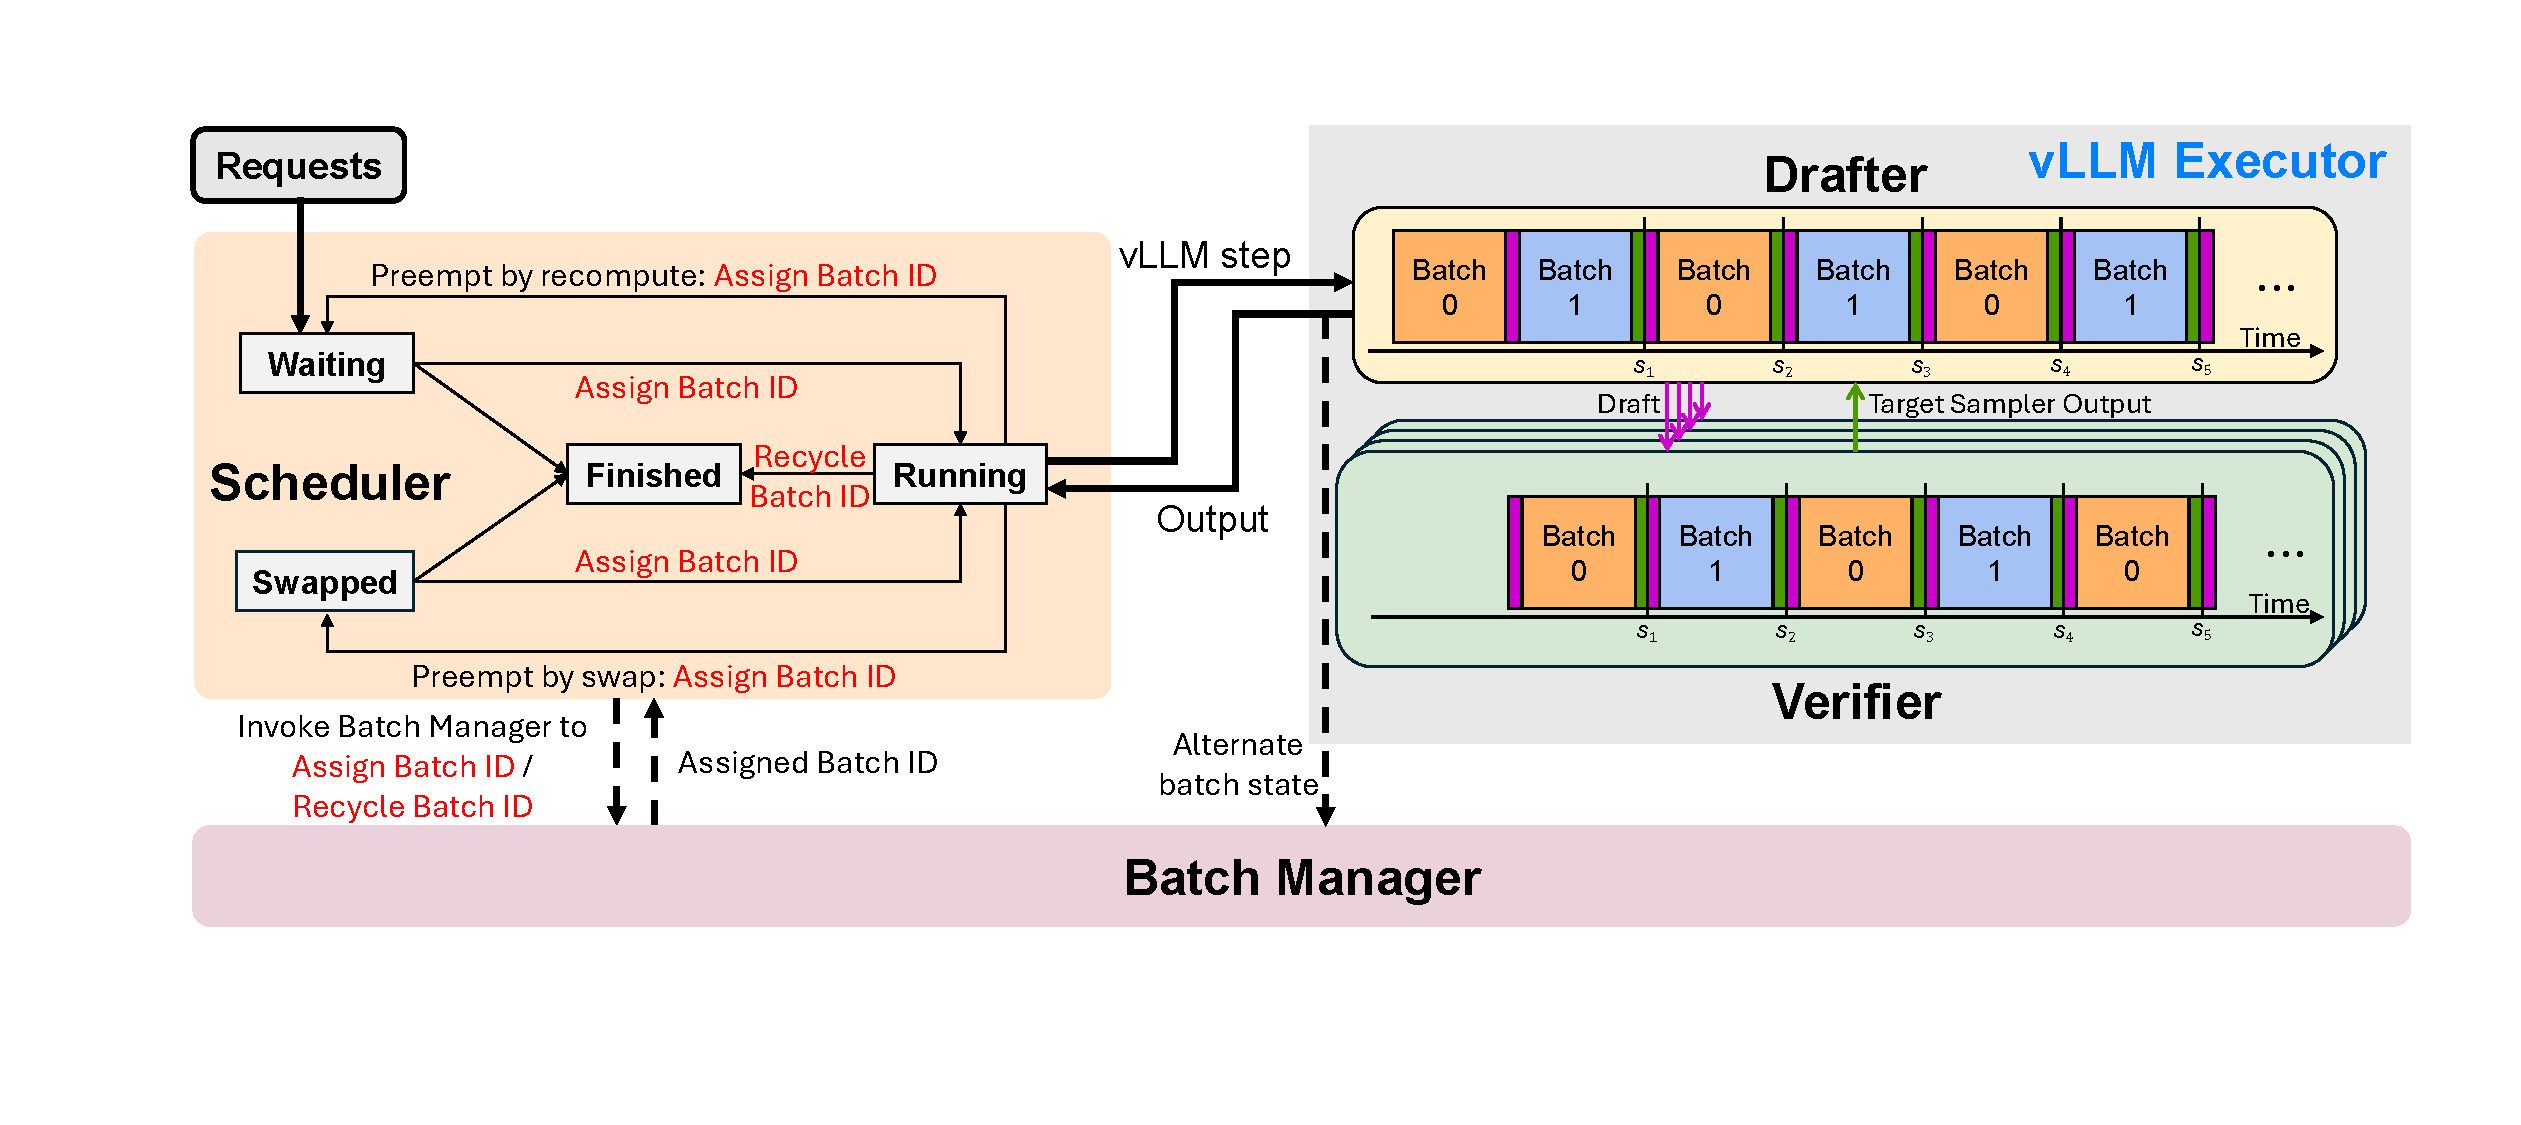
\includegraphics[width=0.96\linewidth]{figures/MineDraft.pdf}
    \caption{
        \textbf{Architecture overview of \alg{}}.
        (Left) The \textbf{Scheduler} manages request life-cycles and batch IDs by coordinating with the \textbf{Batch Manager}, which maintains two batches to enable parallelism in \alg{}.
        (Right) Parallel execution timeline of the \textbf{Drafter} and \textbf{Verifier} across speculative decoding (SD) steps. Magenta blocks/arrows denote broadcast of drafts from the Drafter to the Verifier, while dark green blocks/arrows denote point-to-point dispatch of target sampler outputs from the Verifier to the Drafter. Ticks indicate synchronization points between SD steps. During the initial SD step (before $s_1$), the Drafter sequentially drafts Batch 0, broadcasts drafts to the Verifier, then drafts Batch 1, while the Verifier immediately processes Batch 0 upon receipt and returns outputs to the Drafter. In subsequent SD steps, the two batches alternate roles between drafting and verification, enabling overlapped execution. Batch alternation is triggered when the Drafter returns outputs to the Scheduler at the end of each SD step.  
    }
    \label{fig:overall-arch}
    \vspace{-4mm}
\end{figure*}

Under a mild assumption on $f$, we have the following result.
\begin{restatable}{thm}{ratio}
    \label{thm:ratio}
    Let $W$ be the Lambert $W$ function and $f(t) = 1 - e^{-\alpha t}$ for some constant $\alpha \in \mathbb{R}^+$. For $\alpha V \geq -W_{-1}(-\frac{1}{2e})-1 \approx 1.68$, we have $T_{\SD} > 1.59\ T_{\PSD}$.
\end{restatable}
This result shows that when either the verification time or the curvature of $f$ (captured by $\alpha$) is sufficiently large, PSD achieves at least a $(1.59 - 1)/1.59 > 37\%$ reduction in inference time compared to standard SD.
Since the larger values of $\alpha$ yield stronger diminishing returns in the verification success rate, the product $\alpha V$ can be interpreted as a proxy for the expected number of accepted tokens per step. 
From this perspective, any method with an improved Pareto frontier for $f$ leads to more accepted tokens per step and therefore makes PSD more effective relative to SD.
Finally, note that the naive upper bound on the improvement is $50\%$, corresponding to the idealized case in which drafting is perfectly hidden within the verification time.